%--------------------ELEMENTOS PRÉ-TEXTUAIS--------------------%

%-----------------------------Capa-----------------------------%
\imprimircapa


%------------------------Folha de rosto------------------------%
\imprimirfolhaderosto


%----------------------Ficha Catalográfica----------------------%

% Após a aprovação do trabalho, acesse o link: https://sistemas.uft.edu.br/ficha/

% No formulário do site, preencha os campos desses elementos com os dados do trabalho acadêmico. 
% O programa fará a ordenação e formatação correta dos dados, apresentando a ficha finalizada e normalizada. 
% Faça o download da ficha em formato PDF e salve-a com o nome: ficha_catalografica.pdf
% Substitua o arquivo temporário de mesmo nome presente neste modelo.

\begin{fichacatalografica}
    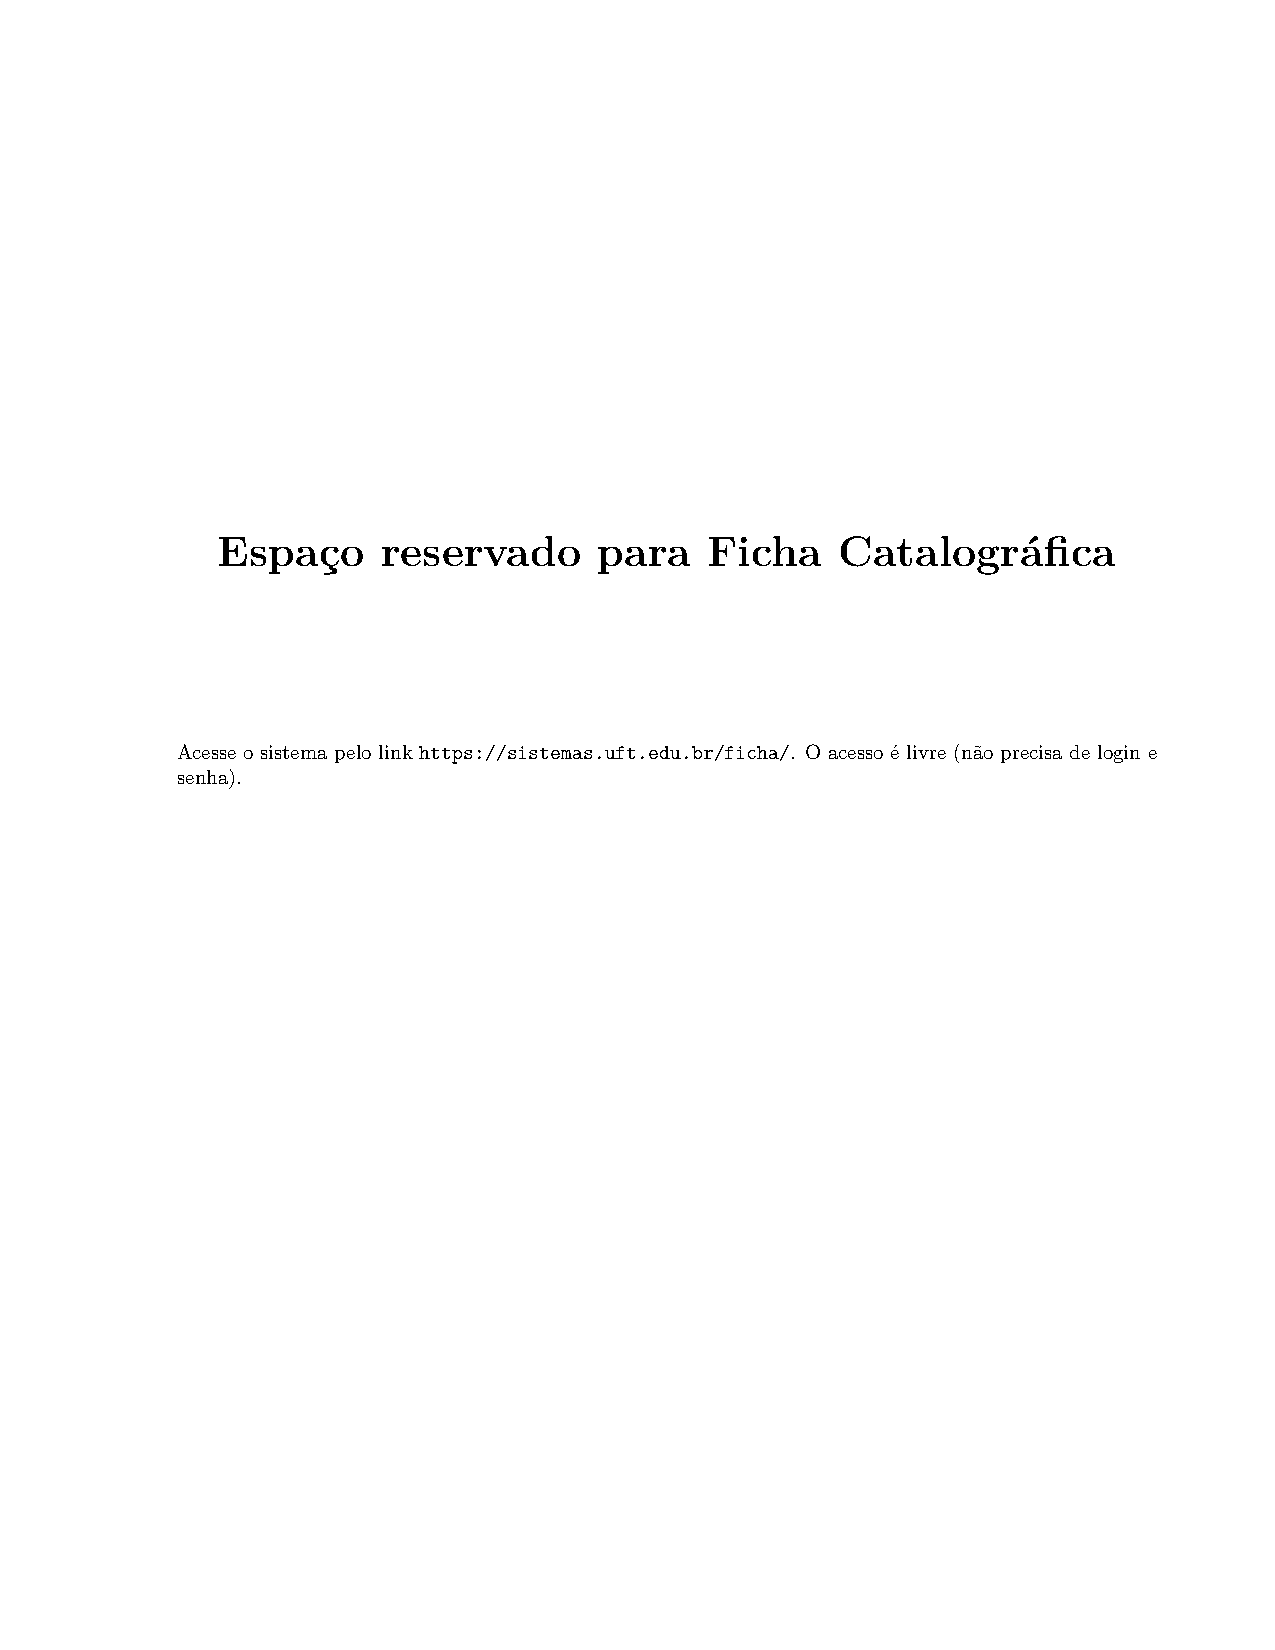
\includepdf{ficha_catalografica.pdf}
\end{fichacatalografica}


%----------------------Folha de Aprovação----------------------%

% Após aprovação do trabalho, solicite do orientador a Folha de Aprovação assinada pela Banca Examinadora.
% Salve-a em formato PDF com o nome: folha_aprovacao.pdf
% Substitua o arquivo temporário de mesmo nome presente neste modelo.

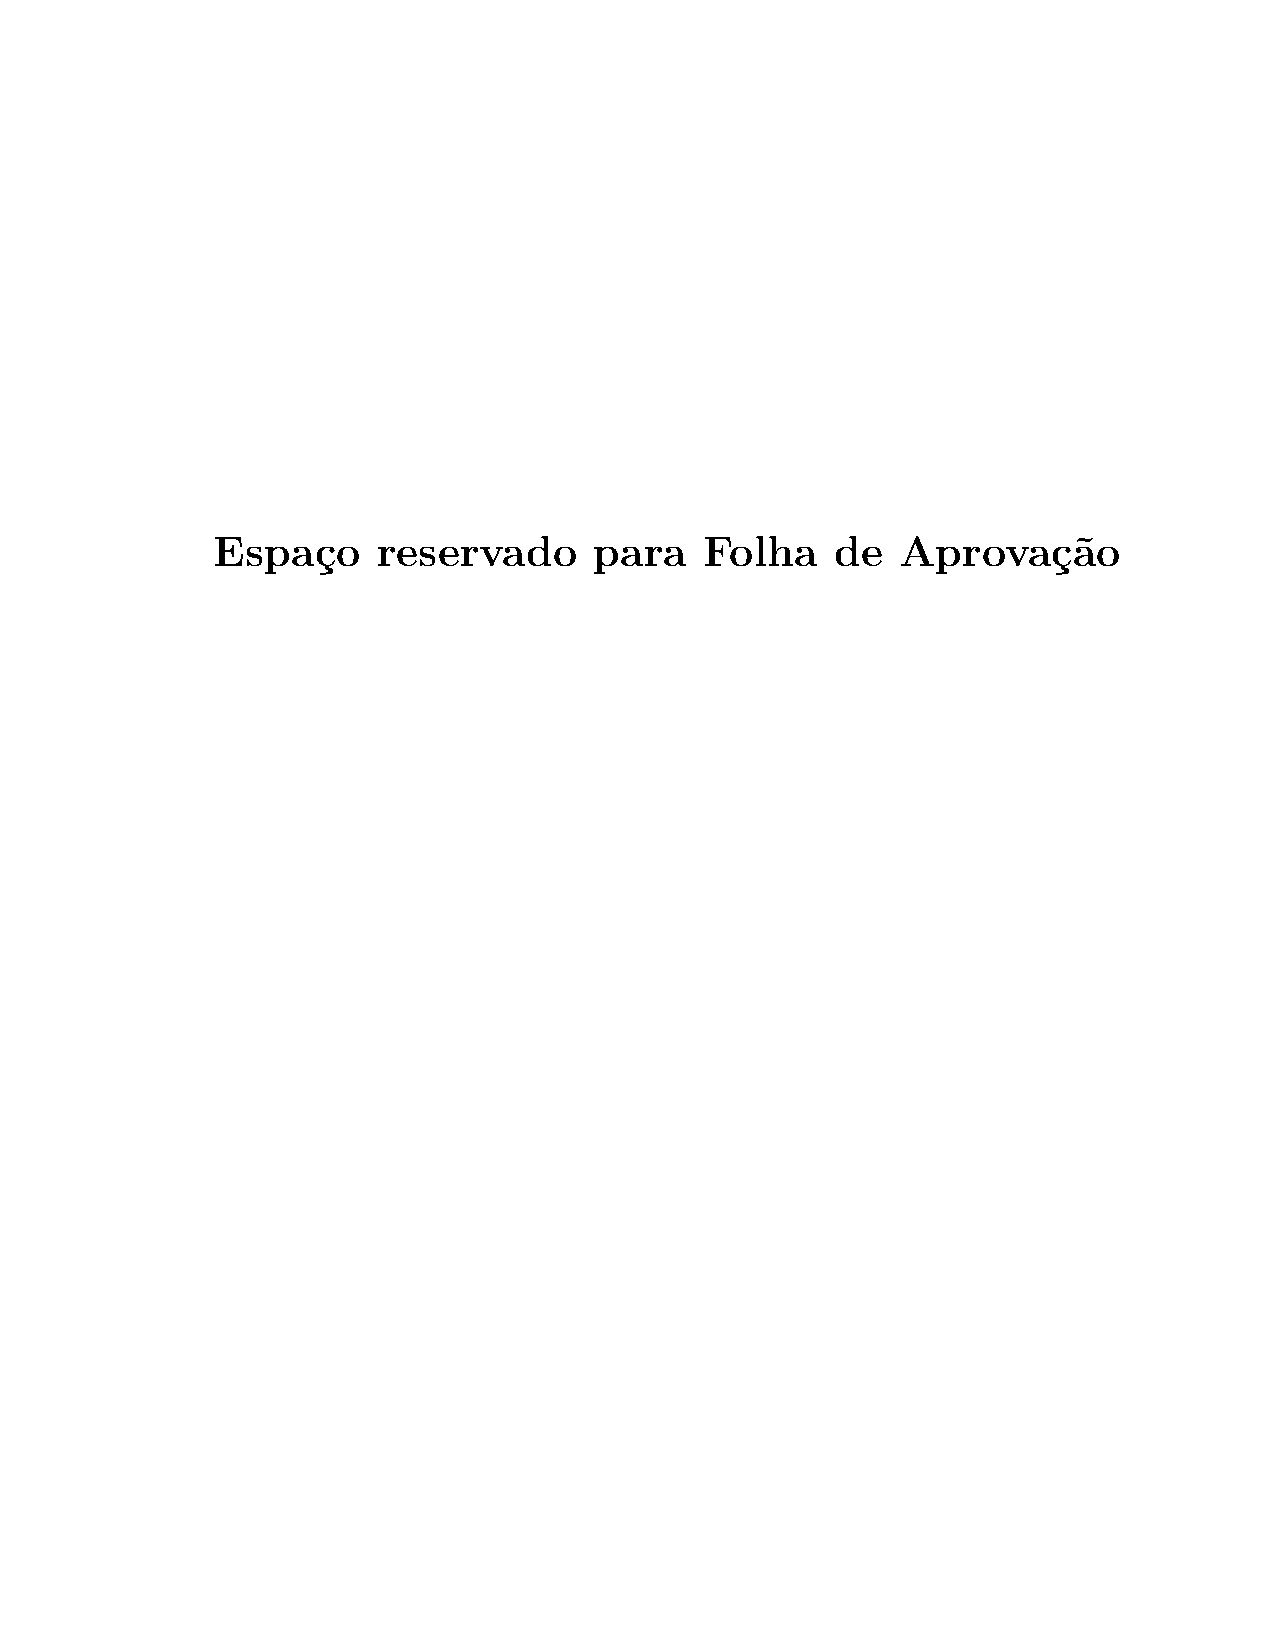
\includepdf{folha_aprovacao.pdf}


%----------------------Dedicatória----------------------%
\begin{dedicatoria}
\vspace*{\fill}
	\begin{flushright}
		\textit{
            A Fulano.\\
   		   A Beltrano.
        }
	\end{flushright}
\end{dedicatoria}


%----------------------Agradecimentos----------------------%
\begin{agradecimentos}

À Universidade Federal do Tocantins (UFT) ...

À Sociedade Brasileira de Matemática (SBM) pela coordenação deste importante programa de mestrado.

Ao meu orientador ...

Aos familiares e amigos ...

\end{agradecimentos}


%----------------------Epígrafe----------------------%
\begin{epigrafe}
    \vspace*{\fill}
	\begin{flushright}
		\textit{
            Um texto interessante.\\
		      (Fulano de Tal)
        }
	\end{flushright}
\end{epigrafe}


%----------------------Resumos----------------------%
%----------------Resumo em Português----------------%
\begin{resumo}
\SingleSpacing

    \noindent Espaço reservado para a escrita do resumo da dissertação. As principais regras para a escrita do resumo encontram-se na norma ABNT 6026 de 2003. De acordo com essa norma, o resumo deve apresentar os pontos maios relevantes da pesquisa: objetivos, os métodos, os resultados, bem como as conclusões. Deve-se evitar o uso de equações, fórmulas, figuras.
    
    \vspace{\onelineskip}
    
    \noindent
    \textbf{Palavras-chave}: palavra-chave1; palavra-chave2; palavra-chave3.
    
\end{resumo}

%----------------Resumo em Inglês----------------%
\begin{resumo}[\textbf{Abstract}]
\SingleSpacing
    \begin{otherlanguage*}{english}
    
        \noindent This is the abstract. This space is reserved for dissertation abstract writing. The main rules for writing are found in ABNT 6026 of 2003. According to this standard, the abstract should be presented and the important points of the research: objectives, methods, results, as well as conclusions. One should avoid using equations, formulas, figures.
        
        \vspace{\onelineskip}
        
        \noindent 
        \textbf{Keywords}: keyword1; keyword2; keyword3.
        
    \end{otherlanguage*}
\end{resumo}


%----------------Lista de Ilustrações----------------%
\pdfbookmark[0]{\listfigurename}{lof}
\listoffigures*
\vspace{-1.35cm}
\listofquadros*
\cleardoublepage

%----------------Lista de Quadros----------------%
%\pdfbookmark[0]{\listofquadrosname}{loq}
%\listofquadros*
%\cleardoublepage

%----------------Lista de Tabelas----------------%
\pdfbookmark[0]{\listtablename}{lot}
\listoftables*
\cleardoublepage


%--------Lista de de abreviaturas e siglas---------%
\begin{siglas}
	\item[ABNT] Associação Brasileira de Normas Técnicas
	\item[IMPA] Instituto de Matemática Pura e Aplicada
	\item[NBR] Norma Brasileira
	\item[SBM] Sociedade Brasileira de Matemática
	\item[SI] Sistema Internacional
	\item[UFT] Universidade Federal do Tocantins
\end{siglas}


%----------------Lista de Símbolos----------------%
\begin{simbolos}
  \item[$ \mathbb{R} $] Conjunto dos números reais
  \item[$ A^{-1} $] Inversa da matriz quadrada $A$
  \item[$ \sum $] Somatório
  \item[$ \dfrac{df}{dx} $] Derivada da função de uma variável $f(x)$ com reação à variável $x$
  \item[$ \dfrac{\partial F}{\partial x_i} $] Derivada parcial da função de várias variáveis $F (x_1, x_2, \ldots)$ com relação à i-ésima variável $x_i$.
  \item[$ \overrightarrow{v} $] Vetor
\end{simbolos}


%----------------SUMÁRIO----------------%
\pdfbookmark[0]{\contentsname}{toc}
\tableofcontents*
\cleardoublepage
